\newpage
\section{Methodology}\label{sec:methodology}

All experiments concerning the data collection and processing were performed at the long-wavelength \ac{mx} beamline I23 at Diamond Light Source, UK. The data collection takes two experimental modes: X-ray diffraction and X-ray tomography. Data processing was also carried out at beamline facilities. %data from crystal samples at the I23 endstation.

\subsection{Diffraction and tomography data collection}

Experiments detailed in this project were collected on protein crystals of: thaumatin, thermolysin, insulin, and proteinase-K. Additional crystals listed in the appendix include chlorite dismutase (Cld) and OmpK36, which were collected on prior to the start of the project.
Sample preparation for in-vacuum data collection followed the standard procedure for I23 detailed by Duman \textit{et al.} (2021) \cite{Duman2021}.

The in-vacuum sample environment contains a cylindrical P12M detector as well as a multi-axis goniometer to enable collection  in multiple orientations; this provides access to high multiplicity and improves data completeness \cite{Finke2016}. The main axis of orientation is \textit{omega} ($\omega$), and the goniometer also has a \textit{kappa} ($\kappa$) and \textit{phi} ($\phi$) angle for re-orientation of crystals. %(illustrated PICTURE)

Each diffraction experiment collected multiple sweeps of 360$\degree$ of data, \textit{i.e.}, a full set of data. The diffraction data was automatically integrated with \textit{DIALS} \cite{Winter2018} which provides the raw intensities, incident vectors, scattering vectors, and goniometer angles.

Following a diffraction experiment, the sample is kept in its in-beam position to immediately start tomography data collection. The order of the experiments is important because radiation damage will affect the higher resolution information first. The assembly for diffraction experiments is shown in the picture of the inside of the vacuum vessel in \cref{fig:vacuum_chamber}, with the position of the system for tomography data collection
shown with dotted lines (D) \cite{Kazantsev2021}.% A tomography camera is integrated into the sample environment to allow for a simple transition between the experimental modes \cite{Kazantsev2021}, as seen in \cref{fig:vacuum_chamber}.

\begin{figure}
    \centering
    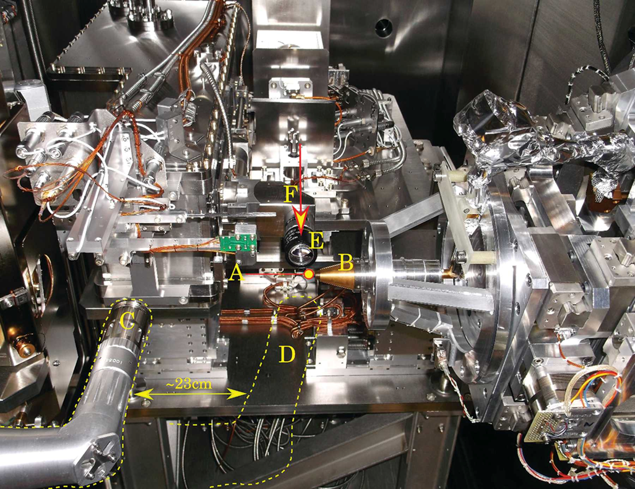
\includegraphics{images/tomo camera.png}
    \caption{A: Sample position; B: goniometer; C: tomography camera in retracted position; D: tomography camera in-beam position; E: viewing system; F: X-ray beam direction. Reproduced from Kazantsev \textit{et al.} (2021) \cite{Kazantsev2021}.}
    \label{fig:vacuum_chamber}
\end{figure}

Diffraction data collection requires the user to specify the energy, rotation increment, image time, and beam transmission. The number of datasets of one crystal corresponds to the diffraction experiments at the same energy using varying orientations of kappa and phi.

Tomography data collection also requires a specified energy, rotation increment, exposure time, and the range of $\omega$ angles to sweep. %While the energy of tomography scans used for the segmentation model does not need to match the experimental diffraction data they are used for, the projection images (also known as flat-fields) should be applied to a dataset with a matching energy. 
To ensure the matching of diffraction and tomography experiments, tomography is collected at every energy that diffraction is collected at, with $\kappa$ and $\phi$ set to zero; this is required for the calculation of absorption coefficients. The tomography collection parameters used in these experiments on the aforementioned crystals are presented in \cref{tomo_table} in the appendix, while the diffraction collection parameters are presented in \cref{diffration_table} in the appendix.

%Further information on the step-by-step procedure of tomography data collection at I23, as used in this work, is detailed in \href{https://confluence.diamond.ac.uk/x/h4HVDQ}{Tomography data collection instructions} on the Diamond Confluence page.

\subsection{Laser-shaping in cryo-crystallography}
% Unibody-Design fs laser
A peripheral lab at Diamond Light Source now houses a commercial femtosecond laser  that has been set up for laser-shaping crystal samples under cryogenic conditions. The product by Light Conversion is a \textbf{CARBIDE-CB5-6W} laser, with a tunable pulse duration between 190 \unit{fs} and 20 \unit{ps}, a maximum power output of 6 \unit{W}, and an air-cooled model. The laser is also installed with the \textbf{2H} \textit{HG for CARBIDE} harmonic generator model by Light Conversion, with output wavelength options of 1030, 515, and 343 \unit{nm}.%of 515 \unit{nm}, mounted on the laser head.
%https://lightcon.com/product/carbide-femtosecond-lasers/#cb5-specifications
%https://lightcon.com/product/harmonic-generator-for-carbide/#specifications

To allow for the swift transfer of samples from a liquid nitrogen bath directly to the liquid nitrogen-cooled goniometer at the femtosecond laser, the laser room used by I23 also houses \href{https://www.diamond.ac.uk/Home/Corporate-Literature/Annual-Review/Review2015/Villages/Macromolecular-Crystallography-Village/Macromolecular-Crystallography-Village-Developments/BART---the-new-robotic-sample-changer-for-MX-beamlines-at-Diamond.html}{BART}, a robotic sample changer for \ac{mx} beamlines at Diamond. The experimental setup allows for samples to be sustained at cryogenic temperatures during transfer and experiment.

\subsection{Data processing pipelines, \textit{DIALS}, and \textit{AnACor}}

Following collection, diffraction data was integrated with \textit{DIALS} for scaling and merging. \textit{DIALS} is one of the standard practice data integration softwares at Diamond Light Source using \ac{sh} to scale reflection data. The scaling and correction of reflections likewise produces merging statistics that provide information on the merged data quality.% $I/ \sigma$ and $R_{merge}$ values.

%Once the merging statistics have been obtained, the reflection data is also produced .
%Further experiments can be run with \href{http://ccp4.github.io/dimple}{Dimple}, an MX pipeline for structure refinement, provided there are anomalous scatterers in the crystal. Using the known \textit{pdb} file of the protein model with the reflection data in an \textit{mtz}, Dimple calculates anomalous density (Anode) peaks from atoms in the structure. The peak heights are affected by several factors, including structural isomerism, binding ions, and water molecules contained in the pdb. While they are not as reliable as merging statistics for assessing the reflection quality, they are used to generate high-resolution electron density maps, as seen in cref{}, which is imperative for MX structure determination.

%The alternative to \textit{DIALS} in generating reflection data is taken using X-ray tomography, which is a longer, multi-step process as it currently entails manually reconstructing the sample model.

The protocol used in the experiments of this project, are an alternative to the standard corrections and scaling performed in \textit{DIALS}; however, the protocol still requires standard processing in \textit{DIALS} in addition to the tomography data processing. 

Tomography data can be visualised in \textit{ImageJ} \cite{Schroeder2020} or in \textit{DAWN} \cite{Basham2015}. After the completion of every tomography scan, the data is processed using the \textit{SAVU} pipeline \cite{Kazantsev2022}. The processing routine here first requires determination of the centre of rotation to align the tomography images; after this is a flat-field correction, followed by ring-artefact removal and reconstruction. Images are also cropped to remove as much background as possible. The flat-field corrected images are an intermediate step in the reconstruction process. Examples of the flat-field corrected images, raw projections, and flat-field corrected projections are presented in \cref{fig:tomo projections}. 

\begin{figure}
    \centering
    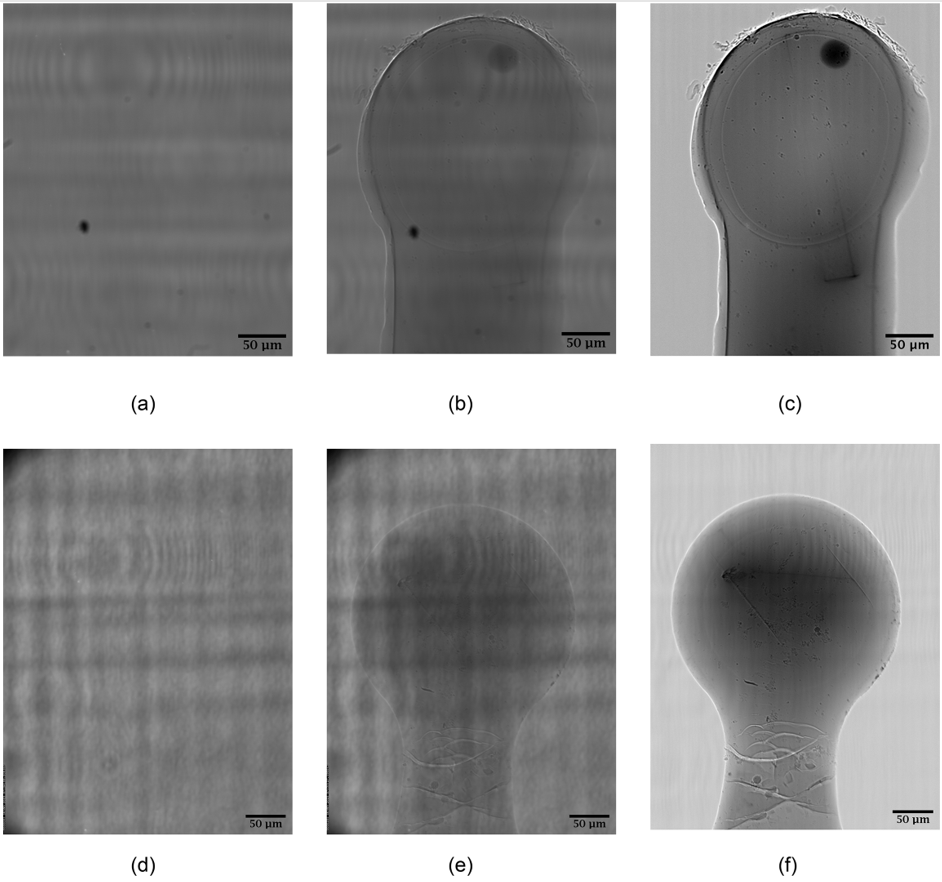
\includegraphics[width = 0.5\textwidth]{images/Tomo projection images CLD and Ompk high quality.png}
    \caption{Tomography projection images of Ompk (top row) and Cld (bottom row) showing: ((a) and (d)) background,  ((b) and (e)) sample, and ((c) and (f)) flat-field corrected images. Produced by Lu \textit{et al.} \cite{Lu2024}.}
    \label{fig:tomo projections}
\end{figure}

The final output from \textit{SAVU} provides reconstructed tomography slices (stacked along the long axis of the sample). Following this, the reconstructed images in the form of 32-bit two-dimensional \textit{tiff} files are converted to 8-bit data to reduce the data size. The reduced data is then imported and manually segmented in the visualisation software Avizo (Thermo Fisher) to distinguish between materials. The segmentation annotates every pixel in each tomography slice to a sample material or to the background, which in turn produces a detailed 3D sample model.

%\begin{figure}
    %\centering
    %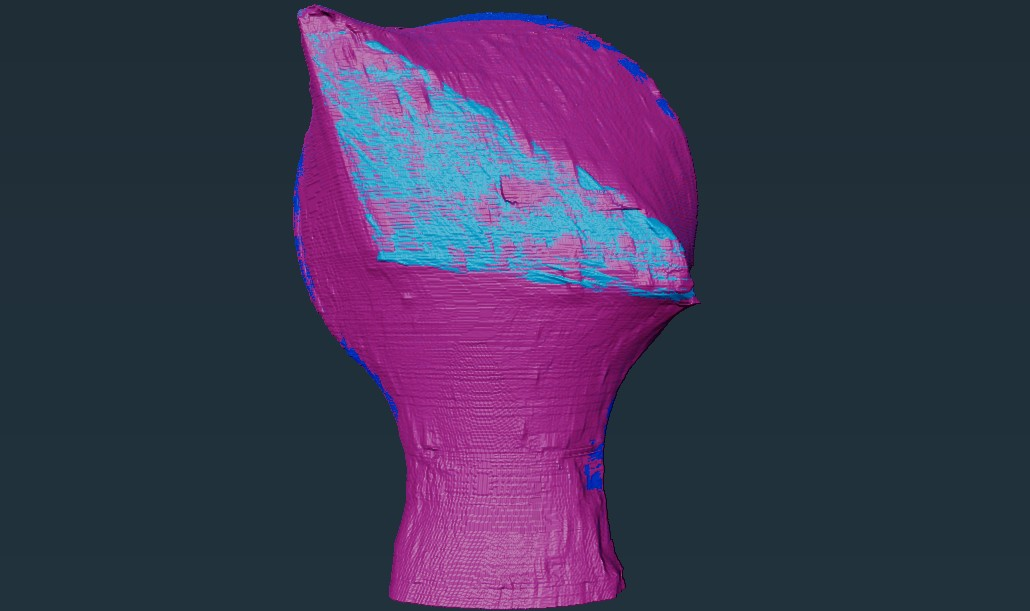
\includegraphics[width = 0.9\textwidth]{images/avizo_flats/cas3_1118.jpg}
    %\caption{3D-segmented model of cryopreserved sample of Cas3 crystal rendered in Avizo; the present materials are crystal (light blue), mother liquor (pink), sample mount (dark blue).}
    %\label{fig:Avizo}
%\end{figure}

The need for segmentation and for flat-field corrected images comes in with \textit{AnACor}, where the X-ray path lengths are traced through the 3D model to calculate absorption coefficients and determine the experimental absorption factors.
%, a ray-tracing software that has been developed collaboratively between I23, Graeme Winter at Diamond Light Source, and Yishun Lu at the Department of Engineering, University of Oxford. AnACor calculates the absorption factors for materials in an analytical 3D model with a discrete form of \cref{AbsFactor}, where the integral over crystal elements $dV$ is replaced with a sum over the crystal voxels $\Delta V$ from  reconstruction \cite{Lu2024}: %applies an analytical absorption correction strategy based on the 3D model of the sample derived from X-ray tomography.

%\begin{equation}
    %A_{\hkl} = \frac{1}{N} \sum_{n=1}^N A_{\hkl}^{(n)}
%\end{equation}
% which visualises provisional 3D models
This happens in two stages in \textit{AnACor}: pre-processing and post-processing. In the pre-processing stage, the intensities from the flat-field corrected images provided are mapped to the corresponding materials in the 3D-segmented model exported from Avizo. The mapping allows for the estimation of absorption coefficients for every material.%and the cropped flat-field images, and feeds these into AnACor to produce a threshold of the sample highlighting where it has high confidence in the presence of a certain percentage of each material. The outcome of pre-processing is a list of absorption factors that are based on where it believes 25\%, 50\%, 75\%, and 100\% of each material lies - this is known as the acceptance percentage. A lower acceptance percentage corresponds to higher confidence, and \textit{vice versa}. % acceptance of the presence

%Absorption factors used in the AnACor experiments were based on 50 \% acceptance of the material, unless stated otherwise.

In the post-processing stage, the absorption coefficients from the prior stage are used to calculate absorption factors, which are then applied to un-corrected reflections from the diffraction experiment. The post-processing step therefore requires the reflection data generated by  \textit{DIALS}. For this reason, the reflection data must be initially produced with  \textit{DIALS}. The output of this stage is the same as in  \textit{DIALS}; reflection data, with data statistics on merging quality - the difference to  \textit{DIALS} is that the two sets of reflection data produced by \textit{AnACor} have been corrected analytically; one with \ac{sh} applied and one without.

Because pre-processing does not generate new reflection data and instead only calculates experimental absorption coefficients, the first stage of the software can also run on samples void of diffracting material, such as an empty loop or a loop containing solvent. The advantage of this is that samples containing only or largely one type of material will produce more reliable coefficients. The outputted values for the non-diffracting materials can then be used in the post-processing of another sample containing the same kind of solvent or loop, as well as the crystal.

Information on the \textit{AnACor} ray-tracing algorithm applied to tomographic reconstructions is described in further detail in Lu \textit{et al.} \cite{Lu2024}.

Provided there are anomalous scatterers of interest in a protein crystal, the reflection data is run through \href{http://ccp4.github.io/dimple}{\textit{Dimple}} \cite{Thorn2011}, an \ac{mx} pipeline for structure refinement. \textit{Dimple}uses the \textit{ANODE} software to calculate anomalous difference Fourier maps, which represent a quality indicator for the anomalous signal in the data. In this process, the reflection data is mapped to a \ac{pdb} format that models the atomic coordinates of the known protein, allowing for the calculation of anomalous density peaks from anomalous groups. The peak heights are affected by several factors, including structural isomerism and binding ions in the \ac{pdb} structure. The Fourier difference maps are the intermediate step to generating electron density maps and are therefore imperative for \ac{mx} structure determination. %While the peaks are not as reliable as merging statistics for assessing the reflection quality, %electron density maps, as seen in cref{}
%MTZ file format is used for the storage of reflection data

\begin{figure}[H]
    \centering
    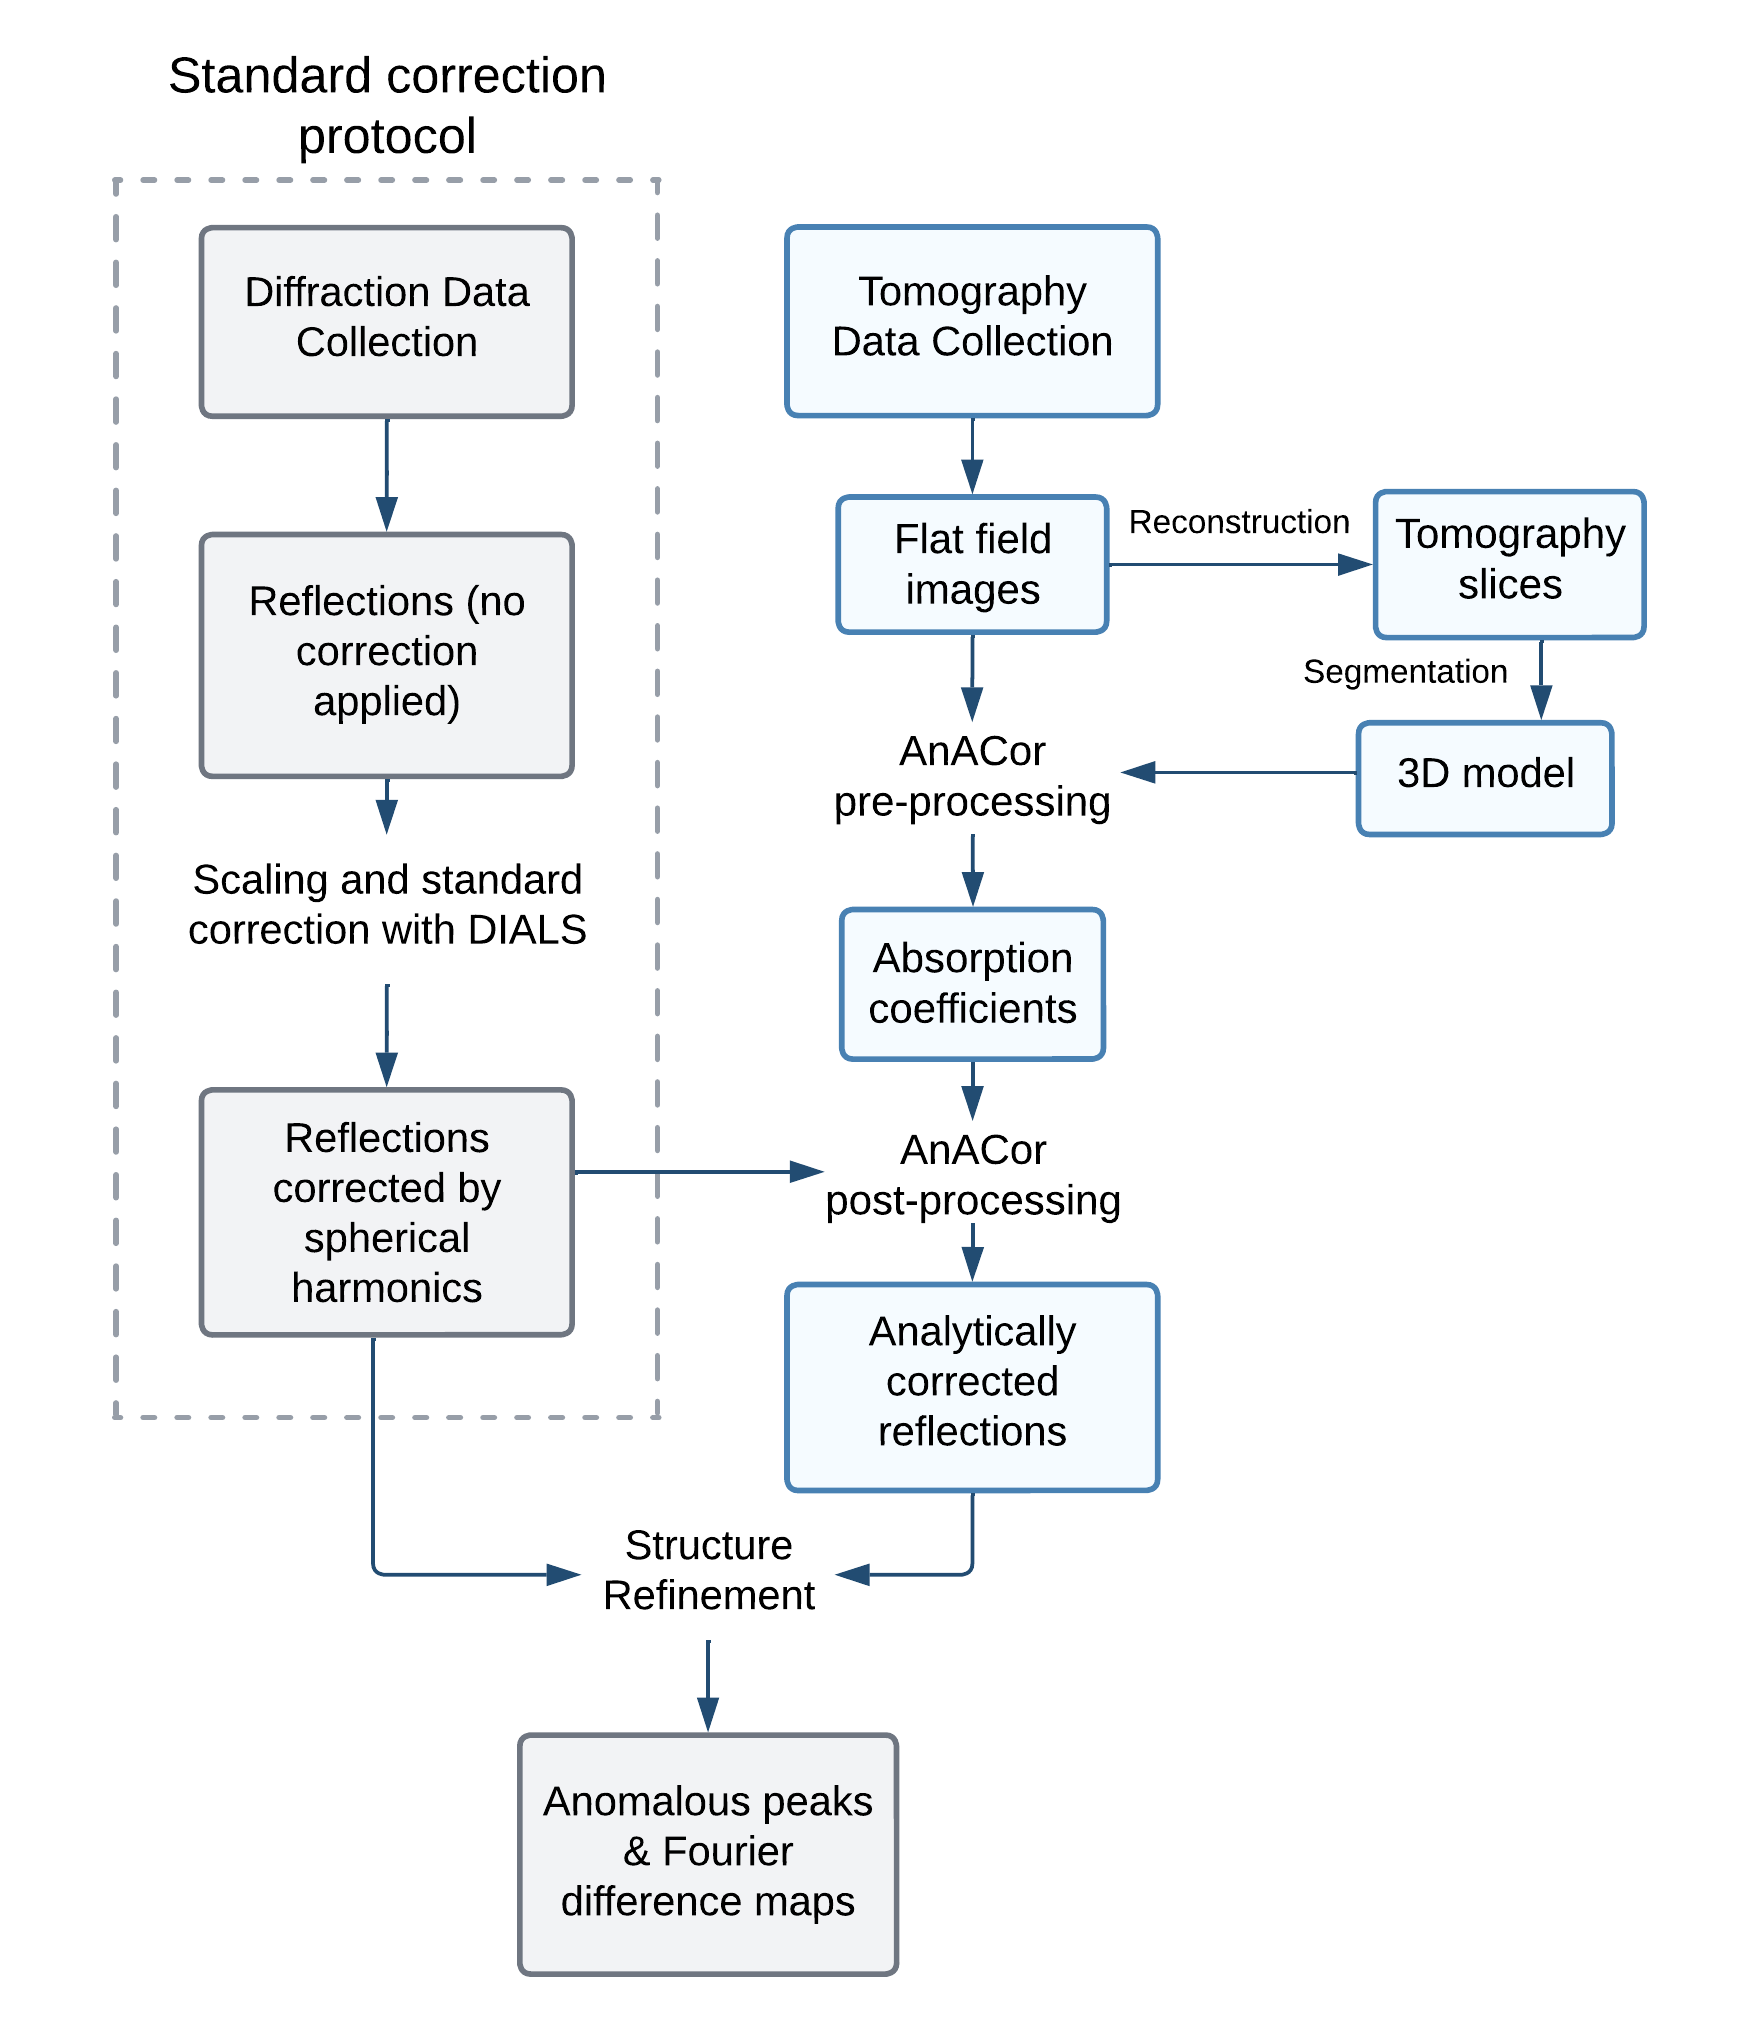
\includegraphics[width = 0.7\textwidth]{images/Tomography Workflow.png}
    \caption{Current workflow of tomography data processing, highlighting the standard protocol for absorption correction using only \textit{DIALS}, and the subsequent protocol needed for analytical absorption corrections with \textit{AnACor}.}
    \label{fig:workflow}
\end{figure}

The typical workflow for the data processing of tomography experiments, as well as the standard  protocol for absorption corrections, is presented in \cref{fig:workflow}.% More information detailing the step-by-step procedure of this workflow, can be found on Diamond Confluence: \href{https://confluence.diamond.ac.uk/x/yIWuD}{Tomography data processing instructions}. %summarised in cref{}


\subsection{Phenix refinement for ion identification}%$f"$-

Phenix is a comprehensive software package for \ac{mx} structure determination \cite{Adams2011} that includes a software extension known as \textit{phenix.refine}. This platform allows for the refinement of various structural parameters, including the $f'$ and $f"$ for a given atom, based on the reflection data and \ac{pdb} structure provided. Given that absorption and emission are sensitive to both wavelength and to the molecular environment, the theoretical parameters are unique to every atom. By refining the model against the reflection data while keeping the theoretical $f'$ fixed, the experimental-calculated $f"$ can be used to identify the ion in question. This practice is still in development for the purpose of ion identification and is referred to as $f"$-refinement in this thesis.%and is used for ion identification at I23.

%As described in the methodology, t
The first stage of \textit{phenix.refine} uses the reflection data provided to produce a modified version of the molecular structure in \ac{pdb} format. This updated molecular structure is then used in the second stage with the same reflection data to estimate the theoretical $f'$ and $f"$ values of specified atoms that are believed to be in the structure. In the case of this experiment, $f'$ was fixed to its theoretical value for a given atom and energy, allowing for an experimental $f"$ to be refined over a specified number of cycles. This value is then corroborated with the theoretical value to determine whether the atom type can be correctly identified.% test the ability of identifying atoms of sulphur and zinc in the crystal by determining their $f"$ peak.

\subsection{Merging statistics: R factor, intensities and estimated uncertainties}

When reflection data is scaled, data reduction software such as \textit{DIALS} also provide a range of statistical parameters, including completeness, multiplicity, and reflection intensities. In diffraction experiments, the data quality is usually assessed by the overall $R_{merge}$ factor based on the reflection intensities. The $R_{merge}$ is a measure of the average ratio of the spread of symmetry-equivalent reflection intensities to the estimated value of reflection intensity \cite{Dauter1999}:

\begin{equation}
    R_{merge} = \sum_{\hkl}\sum_i | I_{\hkl,i} - \langle I_{\hkl} \rangle | / \sum_{\hkl} \langle I_{\hkl} \rangle
\end{equation}

The value itself is calculated in different ways across different data reduction programmes. Due to its high dependence on data multiplicity, the $R$ factor is always higher for high-symmetry space groups compared to those in low symmetry. Higher multiplicity in turn leads to improved data quality, but this must also be weighed with the increase in the $R$ factor.

The merging of diffraction data naturally increases data multiplicity, which can be appealing for enhancing the quality of crystals of low-symmetry space groups with low multiplicity. As with any experiment, outliers can occur. This can be the result of incorrectly classified partially and fully recorded reflections. Merging equivalent intensities provides a chance to identify outliers and remove them from a diffraction experiment. This however must be done with a level of scrutiny and a physical reason for the rejection.

Complementary information about the data quality is provided by the ratio of signal intensities to their uncertainties:

\begin{equation}
    I / \sigma = \sum_{\hkl} I_{\hkl}/\sum_{\hkl} \sigma(I_{\hkl})
\end{equation}

Here, the $\sigma$ values are not trivially estimated and are usually computed in data reduction software packages. Correctly estimating intensity uncertainties is crucial for subsequent applications of the data, for instance in phasing, refinement, and the solving of anomalous-atom positions \cite{Dauter1999}.  

The $R_{merge}$ factor and the ratio of intensities to uncertainties were the main data quality indicators used in the assessment of data quality in the experiments of this project, and are referred to as the merging statistics. It was therefore in the interest of the following experiments to maximise the $I / \sigma$ values while minimising the $R_{merge}$ factors. %These were the main parameters used in the assessment of data quality throughout this project.

Two other complementary indicators for assessing diffraction data quality are the resolution and completeness. The data completeness is defined by the number of reflections collected compared to the number of theoretically possible reflections for a given crystal symmetry \cite{Arkhipova2017}. %This could range from ...
Since each reflection contributes to the electron-density map, the completeness heavily determines the quality of maps \cite{Wlodawer2007}.

For experiments in\textit{Dimple}, the anomalous density peak heights are used as an indicator of the anomalous signal, and therefore of the quality of anomalous difference Fourier maps.

To significantly speed up the analysis of results produced by \textit{DIALS}, \textit{AnACor}, and\textit{Dimple}, python scripts were written and complied to automatically extract, store, and plot the merging statistics and relevant anomalous density peaks of a given crystal or set of crystals. The output of these scripts is seen in the figures of the following section.